\section{Ejercicio 02 Creación del cubo}

Utilice la base de datos AdventureWorksDW2012 como origen de datos
	\begin{center}
	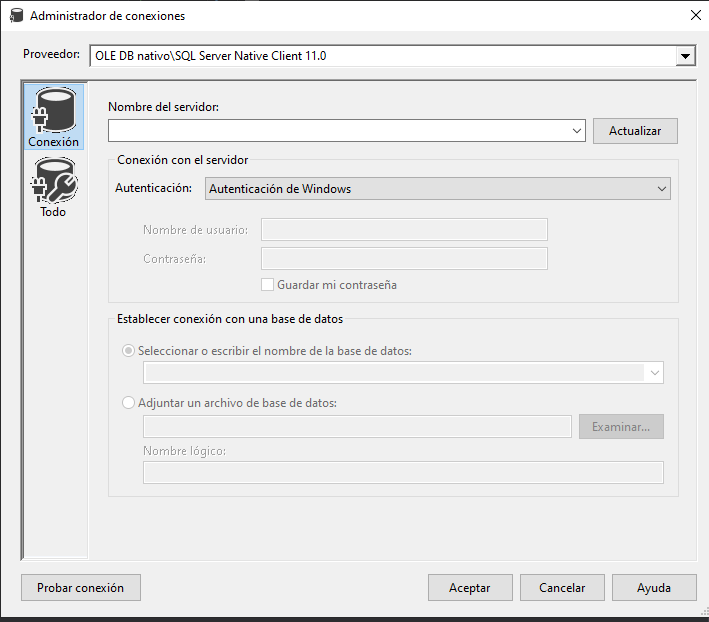
\includegraphics[width=0.5\textwidth]{images/task2/44}
    \end{center}	
    
En la opción definir una vista del origen de datos seleccione las siguientes tablas de la base de datos:
FactInternetSales, DimCurrency, DimCustomer, DimDate, DimProduct, DimPromotion, DimSalesTerritory
	\begin{center}
	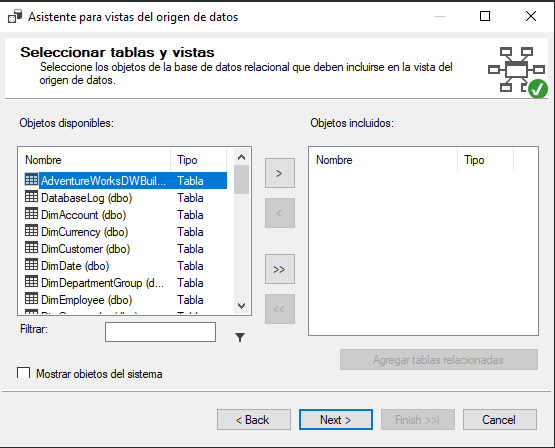
\includegraphics[width=0.5\columnwidth]{images/task2/99}
    \end{center}	
    
Crear un cubo tomando en cuenta las tablas del origen de datos
	\begin{center}
	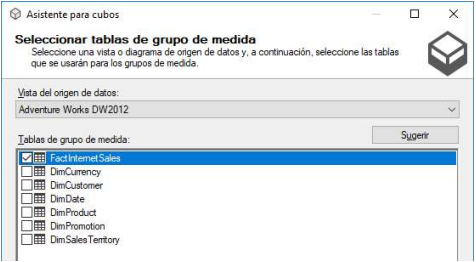
\includegraphics[width=0.5\columnwidth]{images/task2/4}
	\end{center}	
	
	\begin{center}
	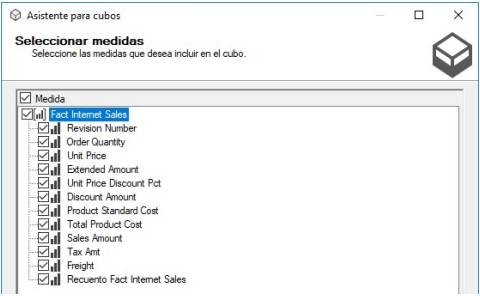
\includegraphics[width=0.5\columnwidth]{images/task2/5}
	\end{center}
	
Procesar el cubo  Examinar el cubo  Cambiar la dimensión Date a:
	\begin{center}
	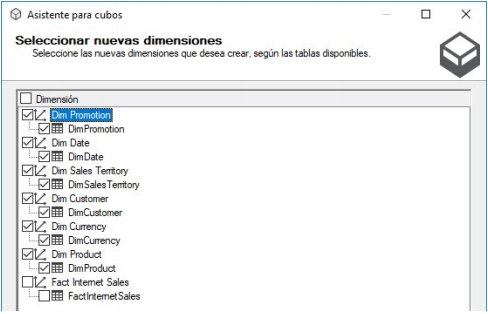
\includegraphics[width=0.5\columnwidth]{images/task2/55}
	\end{center}	

\section{Ejercicio 03 Agregar un cálculo con nombre}

Haga clic en la carpeta Vistas del origen de datos en el Explorador de soluciones, después haga doble clic en el
origen de datos Adventure Works DW2012.dsv
En el panel Tablas, haga clic derecho en DimDate y, a continuación, haga clic en
Nuevo cálculo con nombre

	\begin{center}
	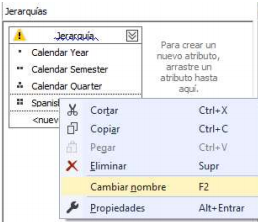
\includegraphics[width=0.25\columnwidth]{images/task2/13}
    \end{center}	
    
En el cuadro de diálogo Crear cálculo con nombre, escriba SimpleDate en el cuadro Nombre de columna y, a
continuación, escriba la siguiente instrucción CASE en el cuadro Expresión:
	\begin{center}
	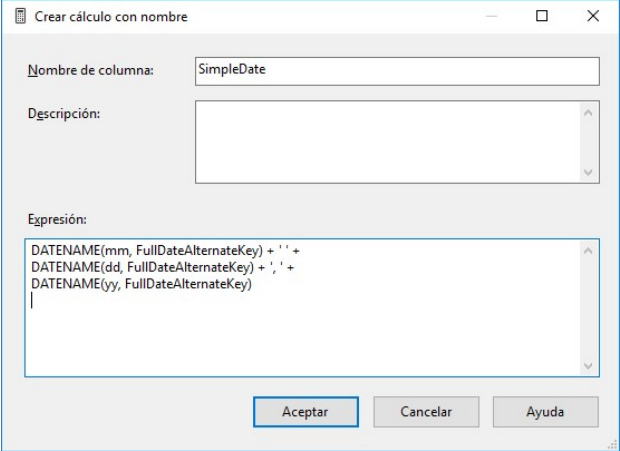
\includegraphics[width=0.5\columnwidth]{images/task2/66}
    \end{center}	
    
Haga clic en Aceptar y expanda DimDate en el panel Tablas
Aparece el cálculo con nombre SimpleDate, con un icono que indica que se
trata de un cálculo con nombre
	\begin{center}
	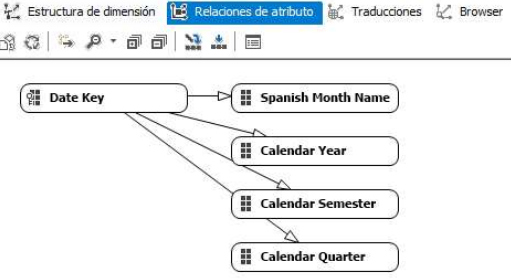
\includegraphics[width=0.5\columnwidth]{images/task2/15}
    \end{center}	
    
En el menú Archivo, haga clic en Guardar todo . 6. En el panel Tablas, haga clic derecho en DimDate y seleccione la opción Explorar datos
Observe que la columna SimpleDate aparece en la vista del origen de datos, concatenando correctamente los
datos de varias columnas del origen de datos subyacente sin modificar el origen de datos original.


	
\section{Ejercicio 04 Usar el cálculo con nombre para los nombres de miembro}

Para utilizar el cálculo con nombre para los nombres de miembro
Haga doble clic en la dimensión DimDate en el nodo Dimensiones del Explorador de soluciones.

	\begin{center}
	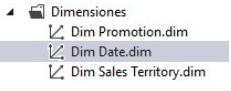
\includegraphics[width=0.25\columnwidth]{images/task2/8}
    \end{center}	

En el panel Atributos de la pestaña Estructura de dimensión, haga clic en el atributo Date Key. Haga clic en el campo de la propiedad NameColumn y, a continuación, haga clic en el botón de puntos suspensivos
(…) para abrir el cuadro de diálogo Columna de nombre.

    
Seleccione SimpleDate en la lista Columna de origen y, a continuación, haga clic en Aceptar.

	\begin{center}
	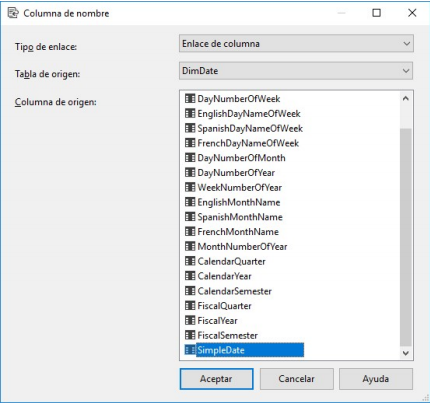
\includegraphics[width=0.5\columnwidth]{images/task2/10}
    \end{center}
    	
\section{Ejercicio 05 Crear una jerarquía}

Para crear una jerarquía
En el Diseñador de dimensiones para la dimensión DimDate, arrastre el atributo Calendar Year del panel
Atributos al panel Jerarquías

	\begin{center}
	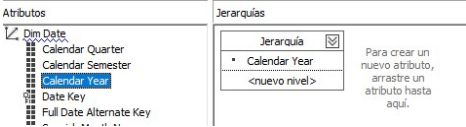
\includegraphics[width=0.5\columnwidth]{images/task2/11}
    \end{center}	
    
Arrastre el atributo Calendar Semester del panel Atributos a la celda <nuevo nivel> del panel Jerarquías, debajo del nivel Calendar Year. 
 Arrastre el atributo Calendar Quarter del panel Atributos a la celda <nuevo nivel> del panel Jerarquías, debajo del nivel Calendar Semester.
 Arrastre el atributo Spanish Month Name del panel Atributos a la celda <nuevo nivel> del panel Jerarquías, debajo del nivel Calendar Quarter. 
 Arrastre el atributo Date Key del panel Atributos a la celda <nuevo nivel> del panel Jerarquías, debajo del nivel
Spanish Month Name.

	\begin{center}
	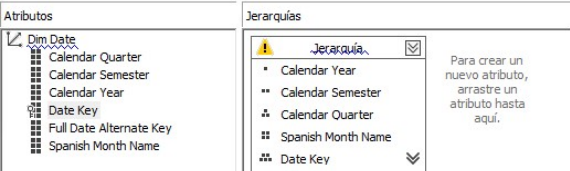
\includegraphics[width=0.5\columnwidth]{images/task2/12}
    \end{center}	

En el panel Jerarquías, haga clic derecho en la barra de título de la jerarquía Jerarquía, seleccione Cambiar nombre
y escriba Calendar Date.
En la jerarquía Calendar Date, cambie el nombre del nivel Spanish Month Name a Calendar Month y el del nivel
Date Key a Date.    
    
    
	\begin{center}
	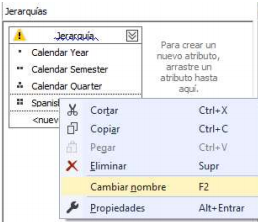
\includegraphics[width=0.25\columnwidth]{images/task2/13}
    \end{center}	       
    
    Elimine el atributo FullDateAlternateKey del panel Atributos, ya que no lo va a usar.
        
	\begin{center}
	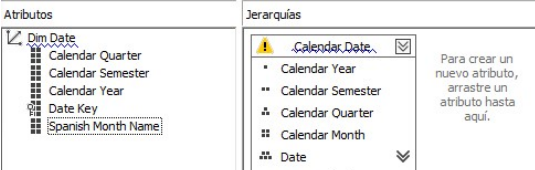
\includegraphics[width=0.5\columnwidth]{images/task2/14}
    \end{center}
    
    Verificar las relaciones del atributo DateKey en la pestaña Realaciones de atributo
        
	\begin{center}
	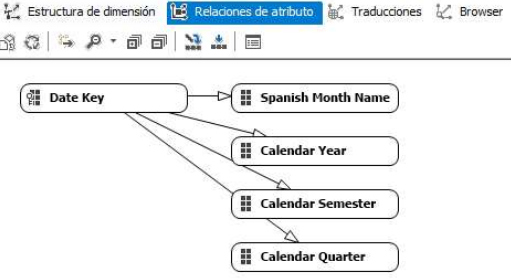
\includegraphics[width=0.5\columnwidth]{images/task2/15}
    \end{center}
